\let\negmedspace\undefined
\let\negthickspace\undefined
\documentclass[journal]{IEEEtran}
\usepackage[a5paper, margin=10mm, onecolumn]{geometry}
%\usepackage{lmodern} % Ensure lmodern is loaded for pdflatex
\usepackage{tfrupee} % Include tfrupee package

\setlength{\headheight}{1cm} % Set the height of the header box
\setlength{\headsep}{0mm}     % Set the distance between the header box and the top of the text

\usepackage{gvv-book}
\usepackage{gvv}
\usepackage{cite}
\usepackage{amsmath,amssymb,amsfonts,amsthm}
\usepackage{algorithmic}
\usepackage{graphicx}
\usepackage{textcomp}
\usepackage{xcolor}
\usepackage{txfonts}
\usepackage{listings}
\usepackage{enumitem}
\usepackage{mathtools}
\usepackage{gensymb}
\usepackage{comment}
\usepackage[breaklinks=true]{hyperref}
\usepackage{tkz-euclide}
\usepackage{listings}
% \usepackage{gvv}
\def\inputGnumericTable{}
\usepackage[latin1]{inputenc}
\usepackage{color}
\usepackage{array}
\usepackage{longtable}
\usepackage{calc}
\usepackage{multirow}
\usepackage{hhline}
\usepackage{ifthen}
\usepackage{lscape}
\renewcommand{\thefigure}{\theenumi}
\renewcommand{\thetable}{\theenumi}
\setlength{\intextsep}{10pt} % Space between text and floats


\renewcommand{\thetable}{\theenumi}

% Marks the beginning of the document
\begin{document}
\bibliographystyle{IEEEtran}

\title{9-9.2-24}
\author{EE24BTECH11048-NITHIN.K}
% \maketitle
% \newpage
% \bigskip
{\let\newpage\relax\maketitle}

\textbf{Question:} \\
Area lying in the first quadrant and bounded by the circle $x^2 + y^2 = 4$ and the lines
x = 0 and x = 2 is \\
\textbf{Solution:} \\
\begin{table}[h!]
      \centering
      \begin{center}
    \begin{tabular}{|c|c|c|} 
        \hline
            \textbf{FUNCTION} & \textbf{FORMULA} \\
        \hline
            $g\brak{x}$ & $\vec{x^TVx}+\vec{2u^Tx}+f=0$ \\
        \hline
	    The points of intersection & $ L: \vec{x} = \vec{h} + \kappa\vec{m}, \kappa \in \mathbb{R} $ \\ of the line L with the conic & $\kappa_i = \frac{1}{\vec{m^TVm}}\brak{\vec{-m^T\brak{Vh+u}} \pm \sqrt{\sbrak{\vec{m^T\brak{Vh+u}}^2} - g(\vec{h})\brak{\vec{m^TVm}}}} $ \\ section as above are \\ given by $ \vec{x}_i = \vec{h} + \kappa_i\vec{m} $ \\
        \hline
    \end{tabular}
\end{center}

      \caption{Variables Used}
\end{table}\\
\text{On comparing g\brak{x} and $x^2 + y^2 - 4 = 0$ the parameters of the circle are} \\
\begin{align}
	\vec{V} = \myvec{ 1 & 0 \\
	0 & 1 } \\
	\vec{u} = \myvec{\frac{0}{0} \\
	0 } \\
	f = -4 \\
\end{align}
\text{The area bounded by $x=0$, $x=2$ and the circle in the first quadrant is} \\
\begin{align}
	\int_{0}^{2}\sqrt{4 - x^2} dx
\end{align}
\text{for indefinite integration of above form we get} \\
\begin{align}
	\int\sqrt{4 - x^2} dx = 2\sin^{-1}\frac{x}{2} + x\sqrt{4 - x^2} + c \\
	2\sin^{-1}\frac{2}{2} + 2\sqrt{4 - 2^2} - 2\sin^{-1}\frac{0}{2} - 0\sqrt{4 - 0^2}
\end{align}
\begin{align}
	\pi
\end{align}
\text{Hence the enclosed area is $\pi$ square units.}
\begin{figure}[h]
\centering
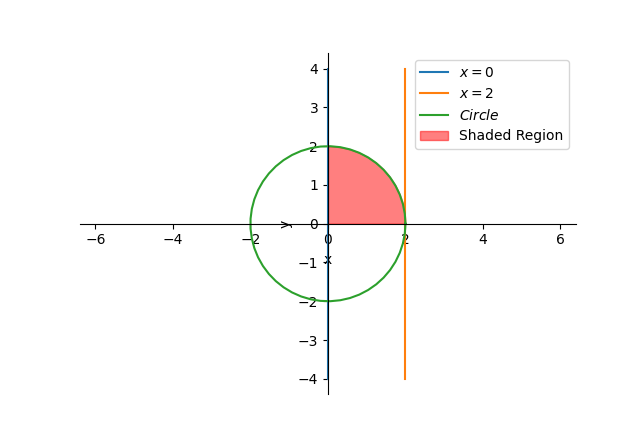
\includegraphics[width=0.7\linewidth]{figs/Figure_1.png}
\caption{Enclosed Area}
\end{figure}
\end{document}
